% CPU
% CPU.tex

\documentclass[12pt,UTF8]{ctexbook}

% 设置纸张信息。
\input{../../../Book/common/page}

% 设置字体，并解决显示难检字问题。
\xeCJKsetup{AutoFallBack=true}
% 注意：ctexbook类已默认设置SimSun为CJKrmdefault
% 以下设置用于确保字体回退和扩展字体可用
% 仅设置扩展字体以避免与默认设置冲突
\setCJKfamilyfont{hei}{SimHei}
\setCJKfamilyfont{kai}{KaiTi}

% 目录 chapter 级别加点（.）。
\usepackage{titletoc}
\titlecontents{chapter}[0pt]{\vspace{3mm}\bf\addvspace{2pt}\filright}{\contentspush{\thecontentslabel\hspace{0.8em}}}{}{\titlerule*[8pt]{.}\contentspage}

% 支持目录点击跳转
\usepackage[colorlinks,linkcolor=blue,citecolor=blue,urlcolor=blue]{hyperref}

% 设置 part 和 chapter 标题格式。
\ctexset{
	part/name= {第,卷},
	part/number={\chinese{part}},
	chapter/name={第,篇},
	chapter/number={\arabic{chapter}}
}

% 图片相关设置。
\usepackage{graphicx}
\graphicspath{{Images/}}

% 设置署名格式。
\newenvironment{shuming}{\hfill\zihao{4}}

% 注脚每页重新编号，避免编号过大。
\usepackage[perpage]{footmisc}

% 设置古文原文格式。
\newenvironment{yuanwen}{\bfseries\zihao{4}}

% 列表项向右偏移。
\usepackage{enumitem}

\usepackage{tabularx}
\usepackage{float}
\usepackage{listings}

\title{\heiti\zihao{0} CPU}
\author{WangFei}
\date{\today}

\begin{document}

\maketitle
\tableofcontents

\frontmatter
\chapter{前言}

本书专为完全没有计算机硬件基础的学习者设计，将带你从零开始了解CPU的基本概念、工作原理和实际应用。

本书将涵盖以下内容：
\begin{itemize}
    \item CPU的基本概念和历史
    \item CPU的内部结构和工作原理
    \item CPU的关键技术和特性
    \item 不同类型CPU的特点和应用场景
    \item CPU的性能指标和选型建议
\end{itemize}

让我们开始这段有趣的学习之旅吧！

\mainmatter

\part{CPU基础概念}

\chapter{什么是CPU}

CPU（Central Processing Unit，中央处理器）是计算机的"大脑"，负责执行程序指令、处理数据。了解CPU的工作原理，对于理解计算机系统的整体运作至关重要。

它具体负责：

\begin{itemize}[leftmargin=2em]
    \item 执行程序指令
    \item 处理和运算数据
    \item 控制计算机各部件协调工作
\end{itemize}

简单来说，CPU就是计算机中负责"思考"和"计算"的部分。

\section{CPU的外观}

CPU通常是一个方形的芯片，大小约几厘米见方。它的特点：

\begin{enumerate}
    \item \textbf{封装形式}：现代CPU大多采用LGA（Land Grid Array）封装，底部有密集的金属触点
    \item \textbf{散热设计}：CPU工作时会产生大量热量，需要安装散热器和风扇
    \item \textbf{针脚/触点}：通过针脚或触点与主板连接，传输电源、数据和控制信号
\end{enumerate}

\begin{figure}[htbp]
    \centering
    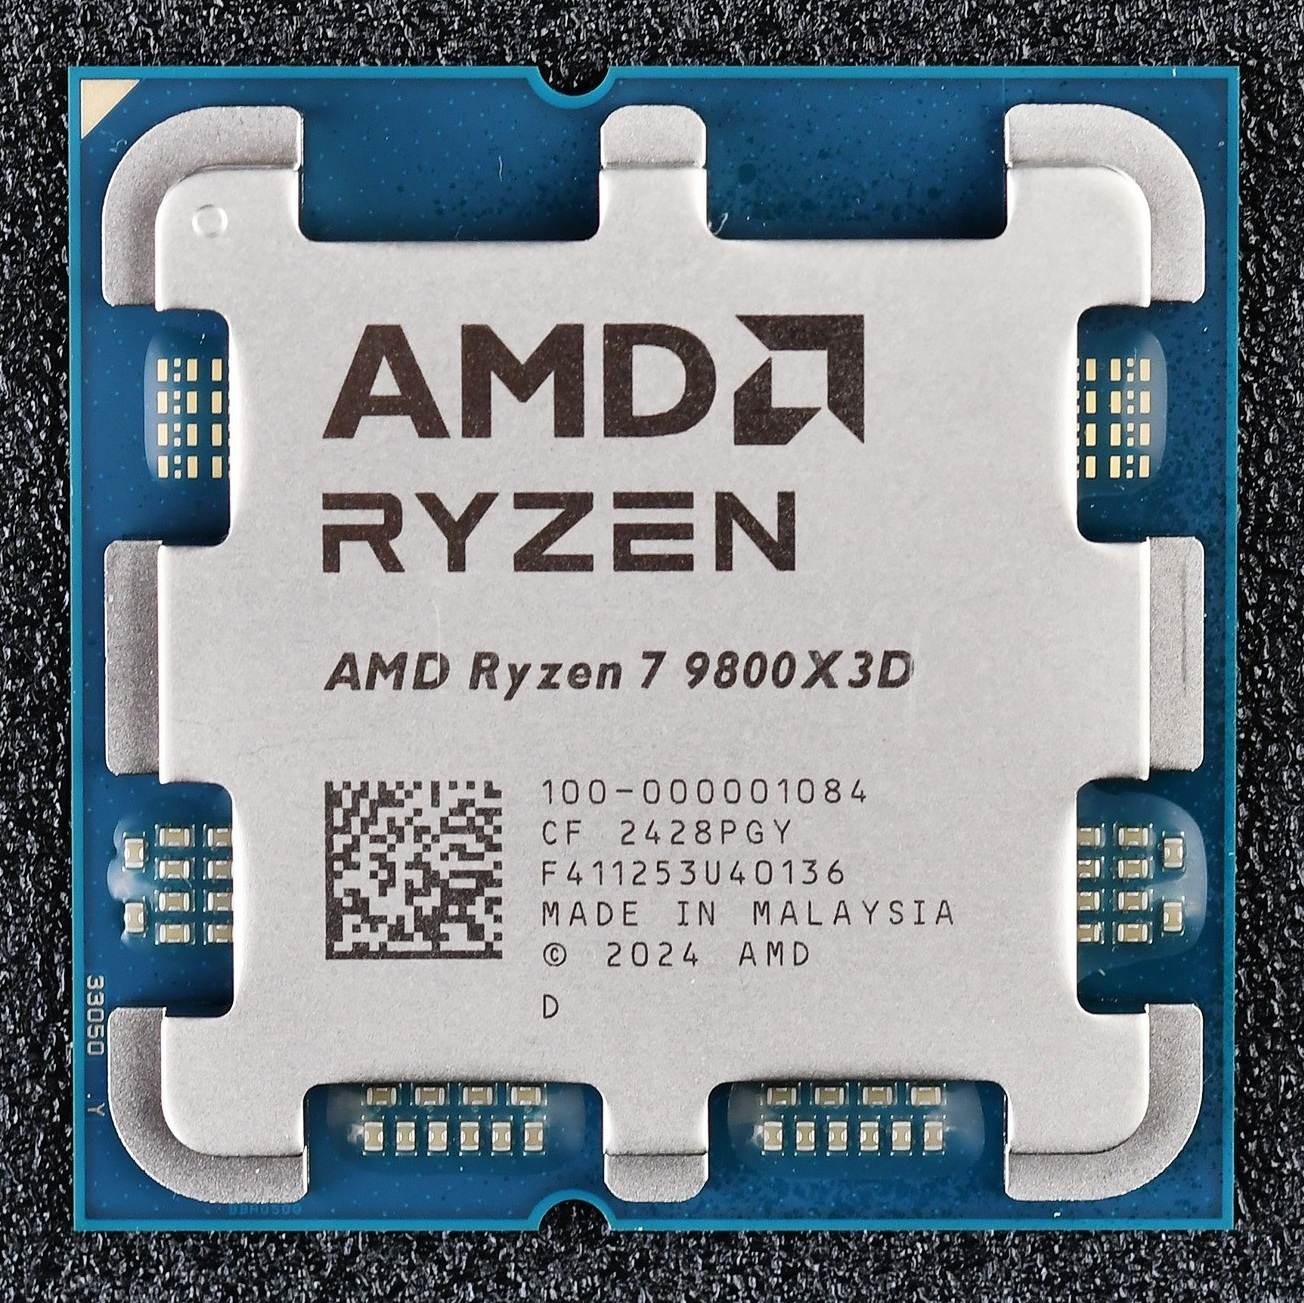
\includegraphics[width=0.5\linewidth]{cpu.jpg}
    \caption{CPU外观}
    \label{fig:cpu外观}
\end{figure}

\section{CPU在计算机中的位置}

在计算机系统中，CPU位于主板上的CPU插槽中：

\begin{itemize}[leftmargin=2em]
    \item 上方：安装散热器和风扇
    \item 周围：内存条、芯片组、扩展插槽等
    \item 通过主板与硬盘、显卡、外设等设备连接
\end{itemize}

\section{CPU的重要性}

CPU的性能直接影响计算机的整体性能：

\begin{itemize}[leftmargin=2em]
    \item \textbf{运行速度}：CPU越快，程序执行越快
    \item \textbf{多任务处理}：强大的CPU可以同时处理多个任务
    \item \textbf{复杂计算}：科学计算、AI训练等需要高性能CPU
\end{itemize}

\chapter{CPU的历史演进}

\section{早期计算机时代}

\begin{enumerate}
    \item \textbf{真空管时代（1940-1950年代）}：
    \begin{itemize}[leftmargin=2em]
        \item 使用真空管作为开关元件
        \item 体积巨大、功耗高、可靠性差
        \item 代表：ENIAC（第一台电子计算机）
    \end{itemize}
    
    \item \textbf{晶体管时代（1950-1960年代）}：
    \begin{itemize}[leftmargin=2em]
        \item 使用晶体管代替真空管
        \item 体积减小、功耗降低、性能提升
        \item 代表：IBM 7090
    \end{itemize}
    
    \item \textbf{集成电路时代（1960年代至今）}：
    \begin{itemize}[leftmargin=2em]
        \item 将大量晶体管集成在一块芯片上
        \item 奠定了现代CPU的基础
    \end{itemize}
\end{enumerate}

\section{x86架构的兴起}

\begin{enumerate}
    \item \textbf{Intel 4004（1971年）}：
    \begin{itemize}[leftmargin=2em]
        \item 世界上第一个商用微处理器
        \item 4位CPU，主频740kHz
        \item 包含2300个晶体管
    \end{itemize}
    
    \item \textbf{Intel 8086（1978年）}：
    \begin{itemize}[leftmargin=2em]
        \item 16位CPU，奠定x86架构基础
        \item 成为IBM PC的核心处理器
    \end{itemize}
    
    \item \textbf{Intel 80386（1985年）}：
    \begin{itemize}[leftmargin=2em]
        \item 32位CPU，支持多任务和虚拟内存
        \item 推动了个人电脑的普及
    \end{itemize}
\end{enumerate}

\section{现代CPU时代}

\begin{enumerate}
    \item \textbf{Pentium系列（1993年起）}：
    \begin{itemize}[leftmargin=2em]
        \item 超标量架构，支持MMX指令集
        \item 开启了CPU性能飞速提升的时代
    \end{itemize}
    
    \item \textbf{多核时代（2005年起）}：
    \begin{itemize}[leftmargin=2em]
        \item 单个CPU集成多个核心
        \item 从双核、四核发展到数十核
    \end{itemize}
    
    \item \textbf{移动与服务器分化}：
    \begin{itemize}[leftmargin=2em]
        \item 移动端：注重低功耗
        \item 服务器端：注重高性能和可靠性
    \end{itemize}
\end{enumerate}

\section{Intel经典产品时间线}

\begin{table}[H]
    \centering
    \begin{tabular}{|p{2cm}|p{5cm}|p{5cm}|}
        \hline
        \textbf{年份} & \textbf{Intel产品} & \textbf{特点} \\
        \hline
        1971 & 4004 & 世界首款商用微处理器，4位 \\
        \hline
        1974 & 8080 & 8位CPU，奠定现代微处理器基础 \\
        \hline
        1978 & 8086 & 16位CPU，x86架构起点 \\
        \hline
        1985 & 80386 & 32位CPU，支持多任务 \\
        \hline
        1989 & 80486 & 集成FPU，性能大幅提升 \\
        \hline
        1993 & Pentium & 超标量架构，MMX指令集 \\
        \hline
        1998 & Xeon & 首款服务器专用CPU，支持多路互联 \\
        \hline
        2000 & Pentium 4 & 长流水线，高频策略 \\
        \hline
        2001 & Xeon MP & 支持4路以上服务器配置 \\
        \hline
        2006 & Core 2 & 双核设计，能效比提升 \\
        \hline
        2006 & Xeon 5000/7000系列 & Woodcrest/Tigerton，双核服务器CPU \\
        \hline
        2008 & Core i7 & Nehalem架构，集成内存控制器 \\
        \hline
        2012 & Xeon E5/E7系列 & Sandy Bridge/Ivy Bridge，主流服务器平台 \\
        \hline
        2017 & Xeon Scalable & Skylake-SP，全新可扩展平台 \\
        \hline
        2020 & Xeon Ice Lake & 10nm工艺，PCIe 4.0支持 \\
        \hline
        2023 & Xeon Sapphire Rapids & 第三代可扩展，支持DDR5和PCIe 5.0 \\
        \hline
        2023 & Xeon Emerald Rapids & 优化能效，延续LGA4677平台 \\
        \hline
        2024 & Core Ultra & 异构计算，NPU集成 \\
        \hline
        2024 & Xeon Sierra Forest & 能效核服务器CPU，高密度部署 \\
        \hline
        2024 & Xeon Granite Rapids & 性能核服务器CPU，AI优化 \\
        \hline
    \end{tabular}
    \caption{Intel经典CPU产品时间线}
    \label{tab:intel_history}
\end{table}

\section{AMD经典产品时间线}

\begin{table}[H]
    \centering
    \begin{tabular}{|p{2cm}|p{5cm}|p{5cm}|}
        \hline
        \textbf{年份} & \textbf{AMD产品} & \textbf{特点} \\
        \hline
        1975 & AM9080 & 首款8位微处理器 \\
        \hline
        1999 & Athlon & 首款超过1GHz的CPU \\
        \hline
        2000 & Athlon XP & 经典高性能处理器 \\
        \hline
        2003 & Athlon 64 & 首款64位x86处理器 \\
        \hline
        2006 & Phenom & 首款原生四核CPU \\
        \hline
        2011 & FX系列 & 推土机架构，多核心设计 \\
        \hline
        2017 & Ryzen & Zen架构，性能大幅提升 \\
        \hline
        2017 & EPYC 7000 & Naples，首款Zen服务器CPU，32核心 \\
        \hline
        2019 & EPYC 7002 & Rome，Zen2架构，64核心，PCIe 4.0 \\
        \hline
        2020 & Ryzen 5000 & Zen3架构，单核性能飞跃 \\
        \hline
        2021 & EPYC 7003 & Milan，Zen3架构，64核心 \\
        \hline
        2022 & Ryzen 7000 & Zen4架构，DDR5支持 \\
        \hline
        2022 & EPYC 9004 & Genoa，Zen4架构，96核心，PCIe 5.0 \\
        \hline
        2023 & EPYC 9005 & Bergamo，Zen4c能效核，128核心 \\
        \hline
        2024 & Ryzen 8000 & Zen5架构，性能提升 \\
        \hline
        2024 & EPYC Turin & Zen5架构，最多128核心 \\
        \hline
    \end{tabular}
    \caption{AMD经典CPU产品时间线}
    \label{tab:amd_history}
\end{table}

\chapter{CPU的核心组成}

\section{运算器（ALU）}

运算器（Arithmetic Logic Unit，ALU）是CPU的"计算器"：

\begin{itemize}[leftmargin=2em]
    \item \textbf{算术运算}：加、减、乘、除等
    \item \textbf{逻辑运算}：与、或、非、比较等
    \item \textbf{位运算}：移位、掩码等
\end{itemize}

\section{控制器（CU）}

控制器（Control Unit，CU）是CPU的"指挥官"：

\begin{itemize}[leftmargin=2em]
    \item 从内存读取指令
    \item 解码指令含义
    \item 控制各部件执行指令
    \item 协调运算器、寄存器和内存的工作
\end{itemize}

\section{寄存器}

寄存器是CPU内部的高速存储单元：

\begin{itemize}[leftmargin=2em]
    \item \textbf{用途}：临时存储正在处理的数据和指令
    \item \textbf{特点}：速度极快，但容量很小（通常几十个字节）
    \item \textbf{常见类型}：
    \begin{itemize}
        \item 通用寄存器：存储数据
        \item 指令寄存器：存储当前指令
        \item 程序计数器：指向下一条指令地址
    \end{itemize}
\end{itemize}

\section{CPU核心结构示意图}

\begin{figure}[htbp]
    \centering
    % \includegraphics[width=0.8\linewidth]{cpu_structure.png}
    \caption{CPU核心结构示意图（待补充图片）}
    \label{fig:cpu_structure}
\end{figure}

\part{CPU工作原理}

\chapter{指令执行过程}

\section{指令周期}

CPU执行一条指令需要经历以下步骤：

\begin{enumerate}
    \item \textbf{取指令（Fetch）}：
    \begin{itemize}[leftmargin=2em]
        \item 从内存读取指令到指令寄存器
        \item 程序计数器指向下一条指令
    \end{itemize}
    
    \item \textbf{解码（Decode）}：
    \begin{itemize}[leftmargin=2em]
        \item 控制器解析指令含义
        \item 确定需要执行的操作和操作数
    \end{itemize}
    
    \item \textbf{执行（Execute）}：
    \begin{itemize}[leftmargin=2em]
        \item 运算器执行具体运算
        \item 可能需要访问内存获取操作数
    \end{itemize}
    
    \item \textbf{写回（Write Back）}：
    \begin{itemize}[leftmargin=2em]
        \item 将结果写回寄存器或内存
        \item 完成指令执行
    \end{itemize}
\end{enumerate}

\section{指令流水线}

为了提高效率，现代CPU使用流水线技术：

\begin{itemize}[leftmargin=2em]
    \item \textbf{原理}：多条指令重叠执行
    \item \textbf{类比}：像工厂流水线一样，每个阶段同时处理不同指令
    \item \textbf{优势}：提高指令执行吞吐量
\end{itemize}

\section{超标量与乱序执行}

\begin{enumerate}
    \item \textbf{超标量（Superscalar）}：
    \begin{itemize}[leftmargin=2em]
        \item 同一时钟周期执行多条指令
        \item 需要多个执行单元
    \end{itemize}
    
    \item \textbf{乱序执行（Out-of-Order Execution）}：
    \begin{itemize}[leftmargin=2em]
        \item 不按顺序执行指令
        \item 先执行不依赖前面结果的指令
        \item 提高流水线利用率
    \end{itemize}
\end{enumerate}

\chapter{时钟与主频}

\section{时钟信号}

CPU的工作节奏由时钟信号控制：

\begin{itemize}[leftmargin=2em]
    \item \textbf{时钟频率}：CPU每秒完成的时钟周期数
    \item \textbf{单位}：赫兹（Hz），常见单位：GHz（吉赫兹）
    \item \textbf{作用}：同步CPU各部件的工作
\end{itemize}

\section{主频与性能的关系}

\begin{enumerate}
    \item \textbf{主频越高越好吗？}：
    \begin{itemize}[leftmargin=2em]
        \item 同架构下，主频越高性能越好
        \item 不同架构之间不能直接比较
    \end{itemize}
    
    \item \textbf{多核时代的变化}：
    \begin{itemize}[leftmargin=2em]
        \item 单纯提高主频遇到功耗和散热瓶颈
        \item 转向多核设计提高整体性能
    \end{itemize}
\end{enumerate}

\section{睿频技术}

\begin{itemize}[leftmargin=2em]
    \item \textbf{定义}：CPU在需要时自动提高主频
    \item \textbf{原理}：利用芯片的设计余量
    \item \textbf{条件}：温度和功耗在安全范围内
    \item \textbf{优势}：兼顾性能和能效
\end{itemize}

\chapter{缓存系统}

\section{缓存的重要性}

\begin{enumerate}
    \item \textbf{速度差异}：
    \begin{itemize}[leftmargin=2em]
        \item CPU：纳秒级响应
        \item 内存：百纳秒级响应
        \item 缓存：介于两者之间
    \end{itemize}
    
    \item \textbf{缓存命中率}：
    \begin{itemize}[leftmargin=2em]
        \item CPU在缓存中找到所需数据的概率
        \item 命中率越高，性能越好
    \end{itemize}
\end{enumerate}

\section{缓存层次结构}

\begin{table}[H]
    \centering
    \begin{tabularx}{\textwidth}{|p{3cm}|p{3cm}|p{3cm}|p{5cm}|}
        \hline
        \multicolumn{1}{|c|}{\textbf{缓存级别}} & \multicolumn{1}{c|}{\textbf{容量}} & \multicolumn{1}{c|}{\textbf{延迟}} & \multicolumn{1}{c|}{\textbf{特点}} \\
        \hline
        L1 & 几十KB & 1-2周期 & 最快，每个核心独立 \\
        \hline
        L2 & 几百KB到几MB & 3-10周期 & 较快，通常每个核心独立 \\
        \hline
        L3 & 几MB到几十MB & 10-30周期 & 最慢，所有核心共享 \\
        \hline
    \end{tabularx}
    \caption{缓存层次结构对比}
    \label{tab:cache_hierarchy}
\end{table}

\section{缓存一致性}

\begin{itemize}[leftmargin=2em]
    \item \textbf{问题}：多个核心的缓存可能保存同一数据的不同版本
    \item \textbf{解决方案}：使用缓存一致性协议（如MESI）
    \item \textbf{作用}：确保所有核心看到的数据是一致的
\end{itemize}

\part{CPU关键技术}

\chapter{多核与多线程}

\section{多核处理器}

\begin{enumerate}
    \item \textbf{定义}：单个CPU芯片上集成多个独立核心
    \item \textbf{优势}：
    \begin{itemize}[leftmargin=2em]
        \item 并行处理多个任务
        \item 提高整体性能
        \item 更好地利用现代软件的并行特性
    \end{itemize}
    \item \textbf{常见核心数}：双核、四核、八核、十六核等
\end{enumerate}

\section{超线程技术}

\begin{enumerate}
    \item \textbf{定义}：单个物理核心模拟多个逻辑核心
    \item \textbf{原理}：
    \begin{itemize}[leftmargin=2em]
        \item 在一个核心内维护多个线程的状态
        \item 当一个线程等待时，执行另一个线程
    \end{itemize}
    \item \textbf{优势}：提高CPU利用率
    \item \textbf{标识}：Intel称为Hyper-Threading，AMD称为SMT
\end{enumerate}

\section{多核编程基础}

\begin{itemize}[leftmargin=2em]
    \item \textbf{并发与并行}：
    \begin{itemize}
        \item 并发：多个任务交替执行
        \item 并行：多个任务同时执行
    \end{itemize}
    \item \textbf{线程与进程}：
    \begin{itemize}
        \item 进程：程序的运行实例
        \item 线程：进程内的执行单元
    \end{itemize}
\end{itemize}

\chapter{指令集架构}

\section{什么是指令集}

\begin{itemize}[leftmargin=2em]
    \item \textbf{定义}：CPU能够执行的指令集合
    \item \textbf{作用}：软件与硬件之间的接口
    \item \textbf{分类}：CISC和RISC
\end{itemize}

\section{CISC架构}

\begin{enumerate}
    \item \textbf{全称}：Complex Instruction Set Computing（复杂指令集）
    \item \textbf{特点}：
    \begin{itemize}[leftmargin=2em]
        \item 指令数量多、功能复杂
        \item 单条指令可完成复杂操作
        \item 代表：x86架构
    \end{itemize}
\end{enumerate}

\section{RISC架构}

\begin{enumerate}
    \item \textbf{全称}：Reduced Instruction Set Computing（精简指令集）
    \item \textbf{特点}：
    \begin{itemize}[leftmargin=2em]
        \item 指令数量少、功能简单
        \item 每条指令执行时间短
        \item 适合流水线和并行处理
        \item 代表：ARM、RISC-V
    \end{itemize}
\end{enumerate}

\section{x86与ARM对比}

\begin{table}[H]
    \centering
    \begin{tabularx}{\textwidth}{|p{3cm}|X|X|}
        \hline
        \multicolumn{1}{|c|}{\textbf{特性}} & \multicolumn{1}{c|}{\textbf{x86}} & \multicolumn{1}{c|}{\textbf{ARM}} \\
        \hline
        架构类型 & CISC & RISC \\
        \hline
        主要应用 & 桌面、服务器 & 移动设备、嵌入式 \\
        \hline
        功耗 & 较高 & 较低 \\
        \hline
        性能 & 单核性能强 & 能效比高 \\
        \hline
        生态系统 & 成熟丰富 & 快速发展 \\
        \hline
    \end{tabularx}
    \caption{x86与ARM架构对比}
    \label{tab:x86_vs_arm}
\end{table}

\section{ARM授权模式}

ARM采用IP授权商业模式，主要有三种授权方式：

\begin{enumerate}
    \item \textbf{架构/指令集授权}：
    \begin{itemize}[leftmargin=2em]
        \item 获得指令集架构的完整授权
        \item 可自行设计CPU内核
        \item 典型客户：苹果、华为海思
    \end{itemize}
    
    \item \textbf{处理器IP授权}：
    \begin{itemize}[leftmargin=2em]
        \item 使用ARM设计好的处理器内核
        \item 可配置核数、缓存等参数
        \item 自主进行后端设计（主频、工艺等）
    \end{itemize}
    
    \item \textbf{处理器优化包(POP)授权}：
    \begin{itemize}[leftmargin=2em]
        \item 获得完整的物理实现方案
        \item 在指定代工厂和工艺下生产
        \item 最快上市，灵活性最低
    \end{itemize}
\end{enumerate}

\section{其他常见架构}

\begin{enumerate}
    \item \textbf{MIPS}：
    \begin{itemize}[leftmargin=2em]
        \item 由美普思科技开发的RISC架构
        \item 广泛用于嵌入式系统
        \item 中国龙芯采用MIPS架构
    \end{itemize}
    
    \item \textbf{PowerPC}：
    \begin{itemize}[leftmargin=2em]
        \item IBM主导的RISC架构
        \item 曾用于苹果Mac电脑
        \item 现在主要用于服务器和游戏机
    \end{itemize}
    
    \item \textbf{RISC-V}：
    \begin{itemize}[leftmargin=2em]
        \item 开源指令集架构
        \item 支持32位、64位和128位
        \item 适合定制化设计
    \end{itemize}
\end{enumerate}

\section{x86扩展指令集}

x86架构通过扩展指令集不断增强CPU能力：

\begin{table}[H]
    \centering
    \begin{tabular}{|p{2cm}|p{3cm}|p{6cm}|p{3cm}|}
        \hline
        \textbf{指令集} & \textbf{发布年份} & \textbf{主要功能} & \textbf{支持CPU} \\
        \hline
        MMX & 1996 & 多媒体扩展，64位整数运算 & Intel Pentium MMX+ \\
        \hline
        SSE & 1999 & 流式SIMD扩展，单精度浮点 & Intel Pentium III \\
        \hline
        SSE2 & 2000 & 双精度浮点，128位寄存器 & Intel Pentium 4 \\
        \hline
        SSE3 & 2004 & 复数运算优化 & Intel Pentium 4 Prescott \\
        \hline
        SSSE3 & 2006 & 补充SSE3，增强数据处理 & Intel Core 2 \\
        \hline
        SSE4 & 2007 & 字符串处理，图形加速 & Intel Penryn \\
        \hline
        AVX & 2011 & 高级向量扩展，256位寄存器 & Intel Sandy Bridge \\
        \hline
        AVX2 & 2013 & FMA融合乘加，整数运算扩展 & Intel Haswell \\
        \hline
        AVX-512 & 2017 & 512位寄存器，深度学习优化 & Intel Skylake-SP \\
        \hline
        AMX & 2023 & 高级矩阵扩展，AI推理加速 & Intel Sapphire Rapids \\
        \hline
    \end{tabular}
    \caption{x86扩展指令集发展历程}
    \label{tab:x86_extensions}
\end{table}

\section{ARM扩展指令集}

\begin{table}[H]
    \centering
    \begin{tabular}{|p{2cm}|p{3cm}|p{6cm}|p{3cm}|}
        \hline
        \textbf{指令集} & \textbf{发布年份} & \textbf{主要功能} & \textbf{支持CPU} \\
        \hline
        NEON & 2005 & SIMD扩展，128位寄存器 & ARMv7及以上 \\
        \hline
        SVE & 2018 & 可伸缩向量扩展，可变长度 & ARMv8.2及以上 \\
        \hline
        SVE2 & 2020 & SVE增强，更多数据类型 & ARMv8.5及以上 \\
        \hline
        Cryptography Extensions & 2016 & 硬件加密加速 & ARMv8.2及以上 \\
        \hline
        FP16 & 2016 & 半精度浮点运算 & ARMv8.2及以上 \\
        \hline
    \end{tabular}
    \caption{ARM扩展指令集发展历程}
    \label{tab:arm_extensions}
\end{table}

\section{CPU微架构发展}

\begin{subsection}{Intel微架构}

\begin{table}[H]
    \centering
    \begin{tabular}{|p{2cm}|p{3cm}|p{6cm}|p{3cm}|}
        \hline
        \textbf{架构名称} & \textbf{发布年份} & \textbf{主要特点} & \textbf{代表产品} \\
        \hline
        P6 & 1995 & 超标量架构，乱序执行 & Pentium Pro \\
        \hline
        NetBurst & 2000 & 长流水线，高频策略 & Pentium 4 \\
        \hline
        Core & 2006 & 双核设计，短流水线 & Core 2 Duo \\
        \hline
        Nehalem & 2008 & 集成内存控制器，QPI总线 & Core i7 900系列 \\
        \hline
        Sandy Bridge & 2011 & AVX指令集，环形总线 & Core i7 2000系列 \\
        \hline
        Ivy Bridge & 2012 & 22nm工艺，PCIe 3.0 & Core i7 3000系列 \\
        \hline
        Haswell & 2013 & AVX2，FMA，TSX & Core i7 4000系列 \\
        \hline
        Broadwell & 2014 & 14nm工艺，改进能效 & Core i7 5000系列 \\
        \hline
        Skylake & 2015 & 14nm优化，DDR4支持 & Core i7 6000系列 \\
        \hline
        Kaby Lake & 2017 & 14nm++，超高清解码 & Core i7 7000系列 \\
        \hline
        Coffee Lake & 2017 & 六核普及，更多缓存 & Core i7 8000系列 \\
        \hline
        Ice Lake & 2019 & 10nm工艺，Sunny Cove核心 & Core i7 10000系列 \\
        \hline
        Tiger Lake & 2020 & 10nm SuperFin，Xe核显 & Core i7 11000系列 \\
        \hline
        Alder Lake & 2021 & 大小核混合架构，Golden Cove+Gracemont & Core i7 12000系列 \\
        \hline
        Raptor Lake & 2022 & Alder Lake增强，更高频率 & Core i7 13000系列 \\
        \hline
        Meteor Lake & 2023 & 4nm工艺，NPU集成 & Core Ultra 100系列 \\
        \hline
        Arrow Lake & 2024 & 3nm工艺，改进能效 & Core Ultra 200系列 \\
        \hline
    \end{tabular}
    \caption{Intel微架构发展历程}
    \label{tab:intel_microarchitecture}
\end{table}

\end{subsection}

\begin{subsection}{AMD微架构}

\begin{table}[H]
    \centering
    \begin{tabular}{|p{2cm}|p{3cm}|p{6cm}|p{3cm}|}
        \hline
        \textbf{架构名称} & \textbf{发布年份} & \textbf{主要特点} & \textbf{代表产品} \\
        \hline
        K7 & 1999 & 超标量，AMD64指令集 & Athlon \\
        \hline
        K8 & 2003 & 集成内存控制器，HT总线 & Athlon 64 \\
        \hline
        K10 & 2007 & 原生多核，共享L3缓存 & Phenom \\
        \hline
        Bulldozer & 2011 & 模块化设计，浮点共享 & FX系列 \\
        \hline
        Piledriver & 2012 & Bulldozer改进，TDP优化 & FX-8350 \\
        \hline
        Steamroller & 2014 & 增强分支预测 & FX-8370 \\
        \hline
        Zen & 2017 & 全新架构，高IPC & Ryzen 7 1000系列 \\
        \hline
        Zen+ & 2018 & 12nm工艺，改进缓存 & Ryzen 7 2000系列 \\
        \hline
        Zen2 & 2019 & Chiplet设计，7nm工艺 & Ryzen 7 3000系列 \\
        \hline
        Zen3 & 2020 & 统一L3缓存，单CCD设计 & Ryzen 7 5000系列 \\
        \hline
        Zen4 & 2022 & 5nm工艺，AVX-512支持 & Ryzen 7 7000系列 \\
        \hline
        Zen4c & 2023 & 能效核，高密度部署 & EPYC Bergamo \\
        \hline
        Zen5 & 2024 & 4nm工艺，性能提升 & Ryzen 7 8000系列 \\
        \hline
    \end{tabular}
    \caption{AMD微架构发展历程}
    \label{tab:amd_microarchitecture}
\end{table}

\end{subsection}

\section{CISC与RISC详细对比}

\begin{table}[H]
    \centering
    \begin{tabularx}{\textwidth}{|p{4cm}|X|X|}
        \hline
        \multicolumn{1}{|c|}{\textbf{对比项}} & \multicolumn{1}{c|}{\textbf{CISC}} & \multicolumn{1}{c|}{\textbf{RISC}} \\
        \hline
        指令系统 & 复杂，数量多 & 精简，数量少 \\
        \hline
        存储器操作 & 控制指令多 & 控制简单 \\
        \hline
        编程效率 & 高，单条指令功能强 & 较低，需要更多指令 \\
        \hline
        CPU芯片电路 & 功能强、面积大、功耗大 & 面积小，功耗低 \\
        \hline
        执行速度 & 单条指令可能较慢 & 单条指令执行快 \\
        \hline
        应用范围 & 通用计算机 & 嵌入式、移动设备 \\
        \hline
    \end{tabularx}
    \caption{CISC与RISC架构对比}
    \label{tab:cisc_vs_risc}
\end{table}

\chapter{虚拟化技术}

\section{什么是虚拟化}

\begin{itemize}[leftmargin=2em]
    \item \textbf{定义}：在物理硬件上创建多个虚拟环境
    \item \textbf{作用}：
    \begin{itemize}
        \item 提高硬件利用率
        \item 隔离不同应用和系统
        \item 便于管理和迁移
    \end{itemize}
\end{itemize}

\section{Intel VT-x}

\begin{enumerate}
    \item \textbf{定义}：Intel的硬件虚拟化技术
    \item \textbf{功能}：
    \begin{itemize}[leftmargin=2em]
        \item VT-x：CPU虚拟化支持
        \item VT-d：设备I/O虚拟化支持
        \item VT-c：网络虚拟化支持
    \end{itemize}
\end{enumerate}

\section{AMD-V}

\begin{enumerate}
    \item \textbf{定义}：AMD的硬件虚拟化技术
    \item \textbf{功能}：
    \begin{itemize}[leftmargin=2em]
        \item AMD-V：CPU虚拟化支持
        \item AMD-Vi：I/O虚拟化支持
    \end{itemize}
\end{enumerate}

\part{CPU分类与选型}

\chapter{CPU的分类}

\section{按用途分类}

\begin{enumerate}
    \item \textbf{桌面CPU}：
    \begin{itemize}[leftmargin=2em]
        \item 用于个人电脑
        \item 平衡性能和功耗
        \item 代表：Intel Core、AMD Ryzen
    \end{itemize}
    
    \item \textbf{服务器CPU}：
    \begin{itemize}[leftmargin=2em]
        \item 用于数据中心服务器
        \item 注重稳定性和可靠性
        \item 支持多路互联和ECC内存
        \item 代表：Intel Xeon、AMD EPYC
    \end{itemize}
    
    \item \textbf{移动CPU}：
    \begin{itemize}[leftmargin=2em]
        \item 用于手机、平板等移动设备
        \item 注重低功耗和能效
        \item 代表：ARM Cortex系列、Apple A系列
    \end{itemize}
\end{enumerate}

\section{按架构分类}

\begin{enumerate}
    \item \textbf{x86架构}：
    \begin{itemize}[leftmargin=2em]
        \item Intel和AMD的主流CPU
        \item 兼容性强，软件生态丰富
    \end{itemize}
    
    \item \textbf{ARM架构}：
    \begin{itemize}[leftmargin=2em]
        \item 广泛用于移动设备
        \item 低功耗、高效率
        \item 正在向服务器领域扩展
    \end{itemize}
\end{enumerate}

\section{国产CPU简介}

近年来，中国在CPU领域取得了显著进展，主要有以下几个方向：

\begin{enumerate}
    \item \textbf{x86架构}：
    \begin{itemize}[leftmargin=2em]
        \item \textbf{海光信息}：获得AMD Zen架构授权，生产x86服务器CPU
        \item \textbf{兆芯}：基于VIA的x86授权，生产桌面和服务器CPU
    \end{itemize}
    
    \item \textbf{ARM架构}：
    \begin{itemize}[leftmargin=2em]
        \item \textbf{华为海思}：自主设计ARM架构CPU，用于手机和服务器
        \item \textbf{紫光展锐}：面向消费电子和物联网的ARM处理器
    \end{itemize}
    
    \item \textbf{MIPS架构}：
    \begin{itemize}[leftmargin=2em]
        \item \textbf{龙芯}：自主研发的MIPS兼容CPU，用于桌面和嵌入式
    \end{itemize}
    
    \item \textbf{RISC-V架构}：
    \begin{itemize}[leftmargin=2em]
        \item \textbf{赛昉科技}：基于RISC-V的高性能处理器
        \item \textbf{平头哥}：阿里巴巴旗下，开发RISC-V芯片
    \end{itemize}
\end{enumerate}

\chapter{CPU选型指南}

\section{选型考虑因素}

\begin{enumerate}
    \item \textbf{用途}：
    \begin{itemize}[leftmargin=2em]
        \item 日常办公：双核或四核即可
        \item 游戏：四核以上，注重单核性能
        \item 专业创作：多核CPU，大缓存
        \item 服务器：多路CPU，ECC内存支持
    \end{itemize}
    
    \item \textbf{预算}：
    \begin{itemize}[leftmargin=2em]
        \item 入门级：性价比优先
        \item 中高端：平衡性能和价格
        \item 旗舰级：顶级性能
    \end{itemize}
    
    \item \textbf{平台兼容性}：
    \begin{itemize}[leftmargin=2em]
        \item 确认主板Socket兼容
        \item 考虑升级空间
    \end{itemize}
\end{enumerate}

\section{不同场景推荐}

\begin{table}[H]
    \centering
    \begin{tabularx}{\textwidth}{|p{3cm}|X|X|}
        \hline
        \multicolumn{1}{|c|}{\textbf{场景}} & \multicolumn{1}{c|}{\textbf{推荐配置}} & \multicolumn{1}{c|}{\textbf{推荐型号}} \\
        \hline
        日常办公 & 双核/四核，低功耗 & Intel i3、AMD Ryzen 3 \\
        \hline
        游戏娱乐 & 六核以上，高主频 & Intel i5/i7、AMD Ryzen 5/7 \\
        \hline
        专业创作 & 八核以上，大缓存 & Intel i9、AMD Ryzen 9 \\
        \hline
        服务器 & 多路CPU，ECC支持 & Intel Xeon、AMD EPYC \\
        \hline
    \end{tabularx}
    \caption{不同场景CPU推荐}
    \label{tab:cpu_recommendations}
\end{table}

\part{性能与实践}

\chapter{CPU性能指标}

\section{核心性能指标}

\begin{enumerate}
    \item \textbf{核心数/线程数}：
    \begin{itemize}[leftmargin=2em]
        \item 核心数：物理核心数量
        \item 线程数：逻辑核心数量（支持超线程时大于核心数）
    \end{itemize}
    
    \item \textbf{主频/睿频}：
    \begin{itemize}[leftmargin=2em]
        \item 主频：默认工作频率
        \item 睿频：动态提升的最高频率
    \end{itemize}
    
    \item \textbf{缓存大小}：
    \begin{itemize}[leftmargin=2em]
        \item L1/L2/L3缓存容量
        \item 越大越好，影响性能
    \end{itemize}
    
    \item \textbf{TDP功耗}：
    \begin{itemize}[leftmargin=2em]
        \item 热设计功耗
        \item 反映CPU的发热和功耗水平
    \end{itemize}
\end{enumerate}

\section{基准测试}

\begin{enumerate}
    \item \textbf{SPEC CPU}：
    \begin{itemize}[leftmargin=2em]
        \item 专业的CPU性能基准测试
        \item 涵盖整数和浮点运算
    \end{itemize}
    
    \item \textbf{Geekbench}：
    \begin{itemize}[leftmargin=2em]
        \item 跨平台基准测试工具
        \item 包含单核和多核测试
    \end{itemize}
    
    \item \textbf{实际应用测试}：
    \begin{itemize}[leftmargin=2em]
        \item 游戏帧率测试
        \item 视频渲染时间
        \item 编译速度测试
    \end{itemize}
\end{enumerate}

\chapter{CPU散热与功耗}

\section{散热系统}

\begin{enumerate}
    \item \textbf{风冷散热}：
    \begin{itemize}[leftmargin=2em]
        \item 使用散热器和风扇
        \item 成本低，安装方便
        \item 适合大多数场景
    \end{itemize}
    
    \item \textbf{液冷散热}：
    \begin{itemize}[leftmargin=2em]
        \item 使用冷却液传递热量
        \item 散热效果更好
        \item 适合高端CPU和超频
    \end{itemize}
\end{enumerate}

\section{功耗管理}

\begin{enumerate}
    \item \textbf{TDP设计}：
    \begin{itemize}[leftmargin=2em]
        \item 确保散热系统能处理最大功耗
        \item 实际功耗可能低于TDP
    \end{itemize}
    
    \item \textbf{节能技术}：
    \begin{itemize}[leftmargin=2em]
        \item Intel SpeedStep
        \item AMD Cool'n'Quiet
        \item 空闲时降低主频和电压
    \end{itemize}
\end{enumerate}

\chapter{CPU发展趋势}

\section{当前发展方向}

\begin{enumerate}
    \item \textbf{异构计算}：
    \begin{itemize}[leftmargin=2em]
        \item CPU+GPU协同工作
        \item 专用AI加速单元
        \item 提高特定任务效率
    \end{itemize}
    
    \item \textbf{Chiplet技术}：
    \begin{itemize}[leftmargin=2em]
        \item 将CPU分成多个小芯片
        \item 提高良率，降低成本
        \item 便于模块化设计
    \end{itemize}
    
    \item \textbf{3D堆叠}：
    \begin{itemize}[leftmargin=2em]
        \item 垂直堆叠芯片
        \item 缩短连线长度
        \item 提高带宽和效率
    \end{itemize}
\end{enumerate}

\section{未来展望}

\begin{enumerate}
    \item \textbf{摩尔定律}：
    \begin{itemize}[leftmargin=2em]
        \item 传统晶体管缩小接近物理极限
        \item 需要新的技术突破
    \end{itemize}
    
    \item \textbf{新架构探索}：
    \begin{itemize}[leftmargin=2em]
        \item RISC-V的兴起
        \item 神经形态计算
        \item 量子计算研究
    \end{itemize}
\end{enumerate}

\part{附录}

\chapter{CPU常见问题解答}

\section{常见问题}

\begin{enumerate}
    \item \textbf{Q: CPU温度多少算正常？}
    \\A: 正常工作温度一般在40-70°C，满载时不超过90°C为宜。
    
    \item \textbf{Q: 如何查看CPU信息？}
    \\A: Windows可使用任务管理器或CPU-Z；Linux可使用cat /proc/cpuinfo。
    
    \item \textbf{Q: 多核CPU一定比单核CPU快吗？}
    \\A: 取决于软件是否支持多线程。单线程任务主要看单核性能。
    
    \item \textbf{Q: 可以更换CPU吗？}
    \\A: 台式机通常可以，但需要主板Socket兼容。笔记本大多不可更换。
\end{enumerate}

\chapter{参考资料}

\begin{itemize}[leftmargin=2em]
    \item Intel官方网站：https://www.intel.com
    \item AMD官方网站：https://www.amd.com
    \item ARM官方网站：https://www.arm.com
    \item CPU基准测试：https://www.spec.org
\end{itemize}

%=================================================================
% 分隔页：以下为原内容（CPU Socket 详细规格）
%=================================================================
\part{原内容：CPU Socket详细规格}

\chapter{CPU Socket}

CPU Socket 是连接 CPU 与主板、构建整个计算与 I/O 拓扑的核心物理与电气枢纽，直接决定了 CPU 数量、内存 / PCIe 通道分配、NUMA 架构与 GPU 互联性能。

\section{核心定义与作用}

CPU Socket（CPU 插槽）是主板上用于安装 CPU 的机械与电气接口，承担三大核心功能：

\begin{itemize}[leftmargin=2em]
  \item 物理固定：提供零插拔力（ZIF）结构，稳定承载 CPU 并保障散热接触。
  \item 电气连接：通过触点 / 针脚实现 CPU 与主板间的电源、时钟、控制信号、高速数据链路（UPI/xGMI、PCIe、内存总线）传输。
  \item 拓扑定义：决定服务器支持的 CPU 路数（单路 / 双路 / 四路）、内存通道数、PCIe 根节点（Root Complex）数量，是服务器 NUMA 与 I/O 架构的基础。
\end{itemize}

\section{主流封装类型}

服务器 CPU 几乎全部采用 LGA，仅嵌入式场景用 BGA。主流封装类型如下：

\begin{table}[H]
  \centering
  \begin{tabularx}{\textwidth}{|p{4.5cm}|X|X|X|}
    \hline
    \multicolumn{1}{|c|}{\textbf{类型}} & \multicolumn{1}{c|}{\textbf{触点 / 针脚位置}} & \multicolumn{1}{c|}{\textbf{特点}} & \multicolumn{1}{c|}{\textbf{服务器应用}} \\
    \hline
    LGA（Land Grid Array） & 针脚在主板 Socket，CPU 底部为平面触点 & 抗弯针、易维护、适合高密度信号 & Intel Xeon 全系列、AMD EPYC（SP3/SP5） \\
    \hline
    PGA（Pin Grid Array） & 针脚在 CPU，Socket 为孔位 & 易弯针、成本低 & 已淘汰，仅早期 AMD 服务器用 \\
    \hline
    BGA（Ball Grid Array） & CPU 底部为焊球，直接焊接主板 & 不可更换、体积小、信号完整性好 & 边缘计算、高密度嵌入式服务器 \\
    \hline
  \end{tabularx}
  \caption{主流CPU封装类型对比}
  \label{tab:cpu_package_types}
\end{table}

\section{Intel主流CPU Socket}

Intel主流服务器CPU Socket型号包括：

\begin{itemize}[leftmargin=2em]
  \item LGA4677（Eagle Stream）
  \item LGA4710 / LGA7529（Xeon 6 系列）
\end{itemize}

\subsection{LGA4677详细规格}

LGA4677（Eagle Stream）的详细规格如下：

\begin{enumerate}
  \item 适用 CPU：Sapphire Rapids、Emerald Rapids（Xeon 4/5 代）
  \item 针脚数：4677
  \item 核心规格：
    \begin{itemize}[leftmargin=2em]
      \item 内存：8 通道 DDR5-4800
      \item PCIe：PCIe 5.0 + CXL 1.1
      \item 互联：双路 UPI 3.0（11.2GT/s）
      \item 功耗：最高 350W+
    \end{itemize}
  \item 定位：当前主流双路 AI / 云 / HPC 服务器标配，支持多 GPU 与 NVSwitch
\end{enumerate}

\begin{figure}[htbp]
  \centering
  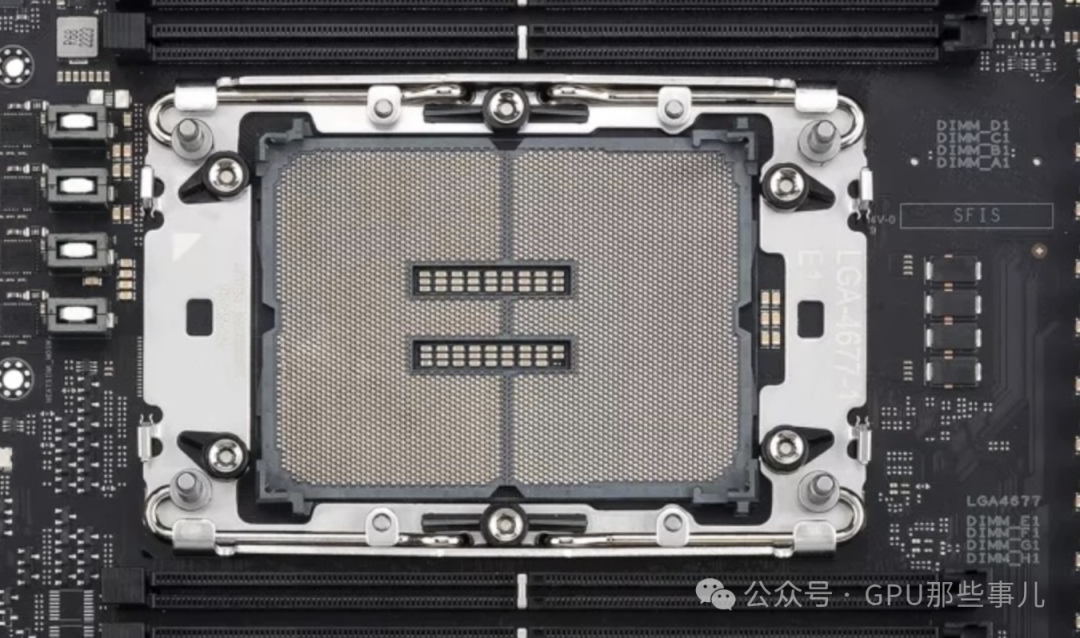
\includegraphics[width=0.7\linewidth]{LGA4677.png}
  \caption{LGA4677（Eagle Stream）Socket}
  \label{fig:lga4677}
\end{figure}

\subsection{LGA4710 / LGA7529详细规格}

LGA4710 / LGA7529（Xeon 6 系列）的详细规格如下：

\begin{enumerate}
  \item 适用 CPU：Sierra Forest（能效核）、Granite Rapids（性能核）
  \item 针脚数：4710 / 7529
  \item 核心规格：
    \begin{itemize}[leftmargin=2em]
      \item 内存：12 通道 DDR5
      \item PCIe：PCIe 5.0 + CXL 2.0
      \item 互联：更高带宽 UPI
    \end{itemize}
  \item 定位：下一代旗舰，面向超大规模数据中心与高密度 AI 训练
\end{enumerate}

\begin{figure}[htbp]
	\centering
	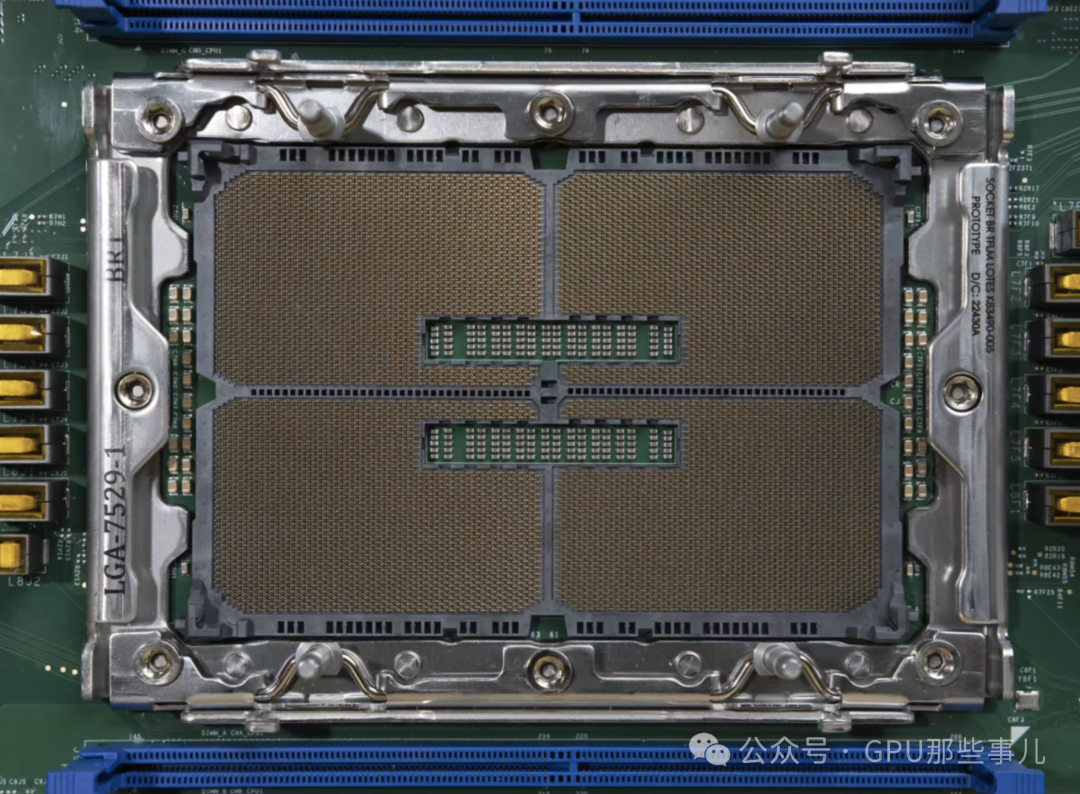
\includegraphics[width=0.7\linewidth]{LGA7529.png}
	\caption{LGA7529（Xeon 6 系列）Socket}
	\label{fig:lga7529}
\end{figure}

\section{AMD主流CPU Socket}

AMD主流服务器CPU Socket型号包括：

\begin{itemize}[leftmargin=2em]
  \item SP5（LGA 6096）
  \item SP3（LGA 4094）
\end{itemize}

\subsection{SP5详细规格}

SP5（LGA 6096）的详细规格如下：

\begin{enumerate}
  \item 适用 CPU：EPYC 9004（Genoa/Bergamo）、9005（Zen5）
  \item 针脚数：6096
  \item 核心规格：
    \begin{itemize}[leftmargin=2em]
      \item 内存：12 通道 DDR5-5200
      \item PCIe：128 条 PCIe 5.0 + CXL 1.1+
      \item 互联：xGMI 3.0
      \item 功耗：最高 400W+
    \end{itemize}
  \item 定位：当前最强服务器 Socket，AI 训练 / 多 GPU 首选
\end{enumerate}

\begin{figure}[htbp]
  \centering
  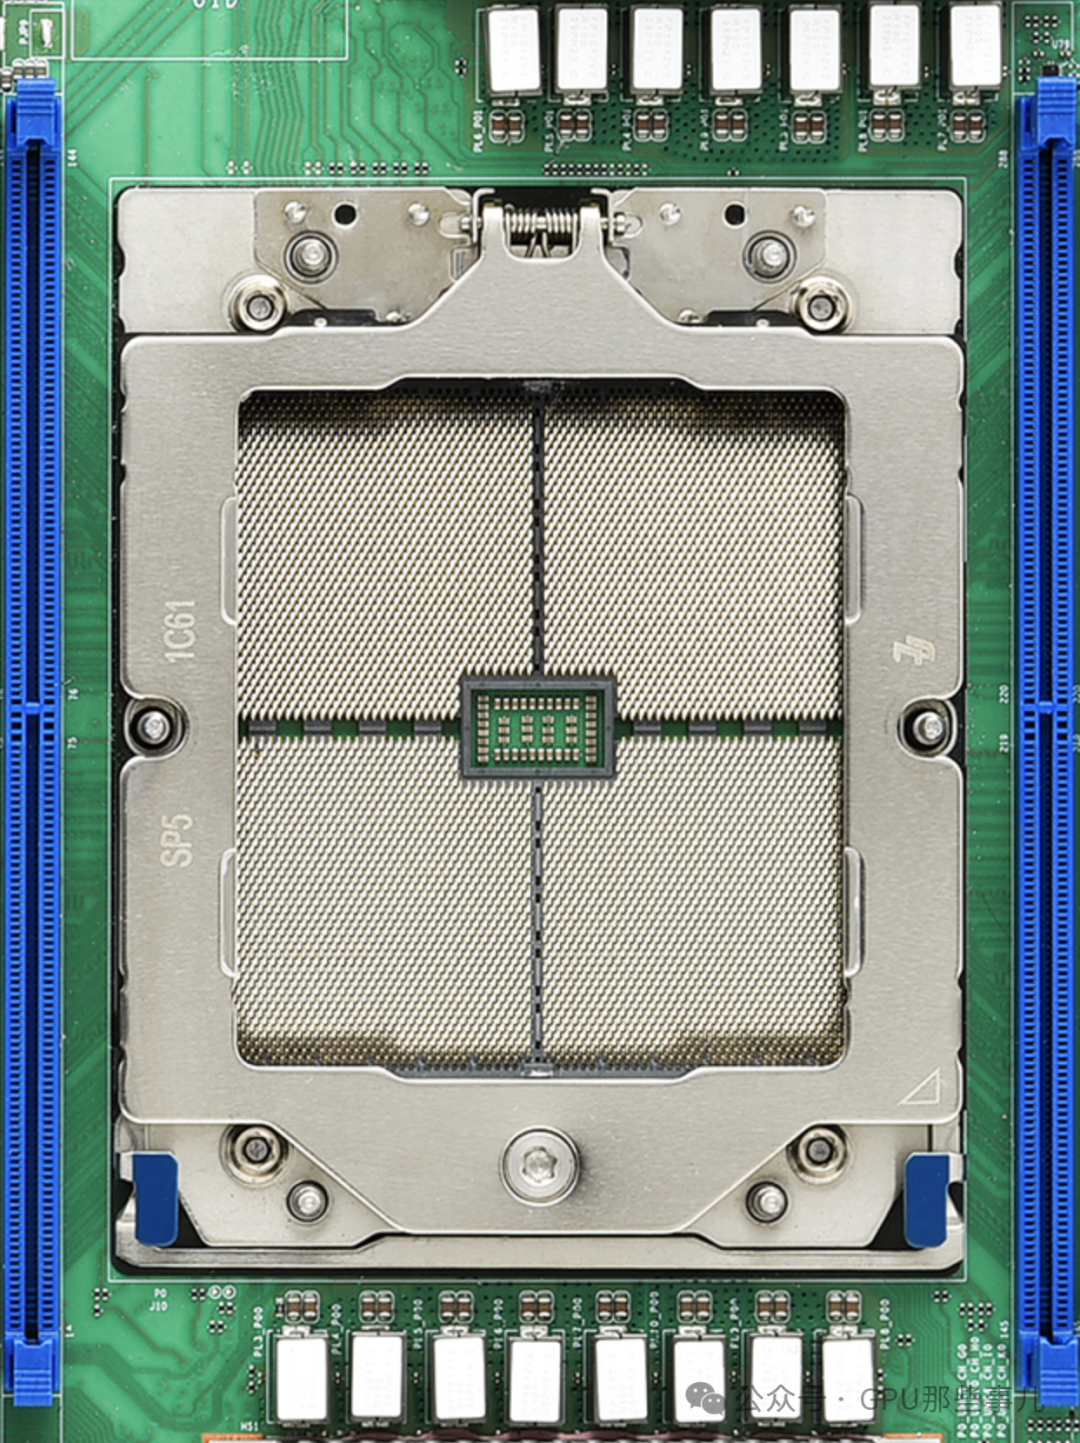
\includegraphics[width=0.7\linewidth]{SP5.png}
  \caption{SP5（LGA 6096）Socket}
  \label{fig:sp5}
\end{figure}

\subsection{SP3详细规格}

SP3（LGA 4094）的详细规格如下：

\begin{enumerate}
  \item 适用 CPU：EPYC 7001/7002/7003（Naples/Rome/Milan）
  \item 针脚数：4094
  \item 规格：PCIe 4.0、DDR4
  \item 定位：存量主流，性价比高
\end{enumerate}

\begin{figure}[htbp]
  \centering
  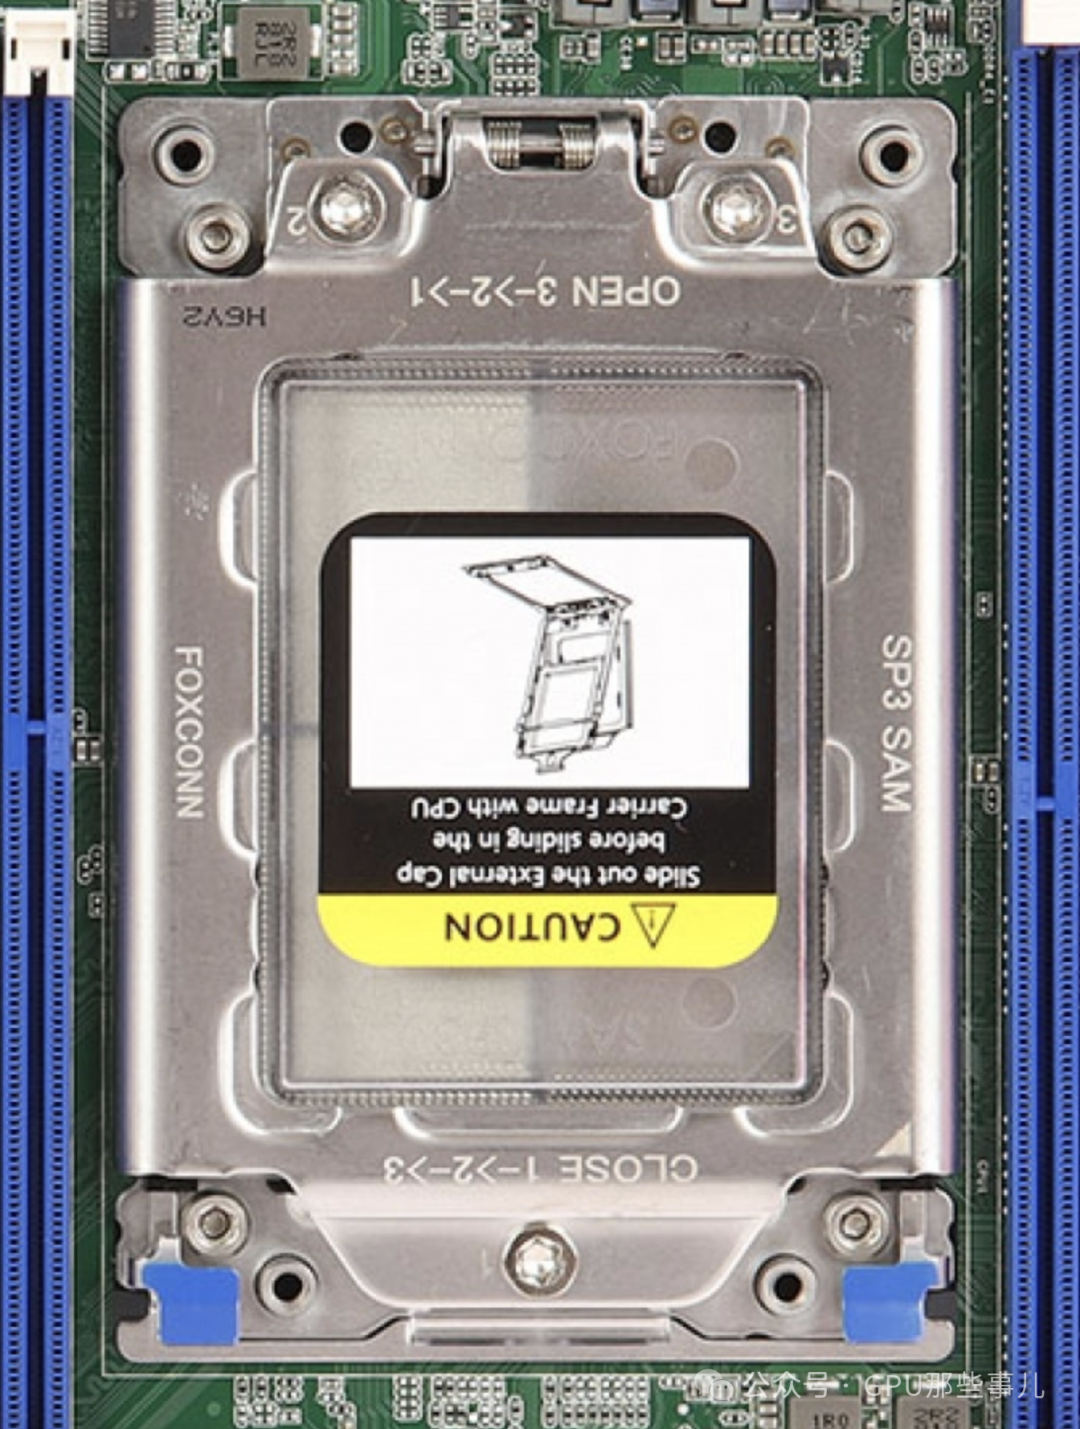
\includegraphics[width=0.7\linewidth]{SP3.png}
  \caption{SP3（LGA 4094）Socket}
  \label{fig:sp3}
\end{figure}

\section{主流CPU Socket规格对比}

\begin{table}[H]
  \centering
  \begin{tabular}{|p{1.5cm}|p{2cm}|p{1.5cm}|p{2.5cm}|p{2.5cm}|p{1.8cm}|p{2cm}|}
    \hline
    \textbf{厂商} & \textbf{Socket} & \textbf{针脚数} & \textbf{内存} & \textbf{PCIe} & \textbf{互联} & \textbf{典型功耗} \\
    \hline
    Intel & LGA4677 & 4677 & 8×DDR5 & 5.0 + CXL & UPI 3.0 & 350W \\
    \hline
    Intel & LGA7529 & 7529 & 12×DDR5 & 5.0 + CXL 2.0 & UPI & 400W+ \\
    \hline
    AMD & SP5 & 6096 & 12×DDR5 & 128×5.0 + CXL & xGMI 3.0 & 400W+ \\
    \hline
    AMD & SP3 & 4094 & 8×DDR4 & 128×4.0 & xGMI & 280W \\
    \hline
  \end{tabular}
  \caption{主流CPU Socket规格对比（Intel vs AMD）}
  \label{tab:socket_comparison}
\end{table}

\backmatter

\end{document}